\documentclass{article}
%\usepackage{geometry}
% \geometry{top = 1in, bottom = 1in, left = 1in, right = 1in}
\usepackage[top = 0.7in, bottom = 0.7in, left = 0.7in, right = 0.7in]{geometry}
\usepackage{amsmath,amssymb,amsthm,mathrsfs}
\usepackage{graphicx}
\usepackage{bm}
\usepackage{float}
\usepackage[font=footnotesize,labelfont=bf]{caption}

\usepackage{fancyhdr}
\pagestyle{fancy}
\rhead{\footnotesize {07/27/2012 ; MESA version 4161} }
\chead{\footnotesize {Authors: Jared Brooks, Lars Bildsten, Bill Paxton} }
\lhead{\footnotesize {mesa/star/test\_suite/irradiated\_planet} }

\begin{document}
	
	\begin{center}
		\begin{Large}
		       \textbf{IRRADIATED PLANET}\\
		\end{Large}
	\end{center}

        This test is to show the evolution of a 0.001 $M_\odot$ (or 1.05 Jupiter Mass) irradiated planet.  The planet receives constant radiation from its host star for 15 Gyr.  This test has two inlists, so the terminal output at the end of the run should read \texttt{``finished all inlists for irradiated\_planet''}.\\

        The first inlist, \texttt{inlist1}, loads the pre-saved model \texttt{very\_low\_mass\_grey\_models/0.001Msun.mod}, and ramps up the  irradiation with the following inlist controls: \texttt{relax\_irradiation = .true. ; relax\_to\_this\_irrad\_flux = 1d7}, and other fine-tuning controls.  It is set to cut off when the surface pressure reaches $10^6$ bar (\texttt{log\_Psurf\_upper\_limit = 6}.  The second inlist, \texttt{inlist2}, turns off the initial irradiation and changes the atmosphere option (\texttt{which\_atm\_option = 'grey\_irradiated'}) which allows controls for irradiation effects, including setting the equilibrium temperature (\texttt{atm\_grey\_irradiated\_T\_eq = 1000}).  This inlist is set to cut off when the age of the model reaches 15 Gyr (\texttt{max\_age = 15d9}).  All of the following plots are generated by the second inlist.\\

        The abundance profile below (figure \ref{fig:1}), with the log mass fraction plotted against q, where q is the fraction of star mass interior to outer boundary of each zone, moving outwards from the core, shows that the planet is fully convective and composed of mainly hydrogen and helium.  The plot to the right (figure \ref{fig:2}) shows the planet contracting throughout its evolution.

	\begin{figure}[H]
                \begin{minipage}[b]{0.5\linewidth}
		       \centering
		       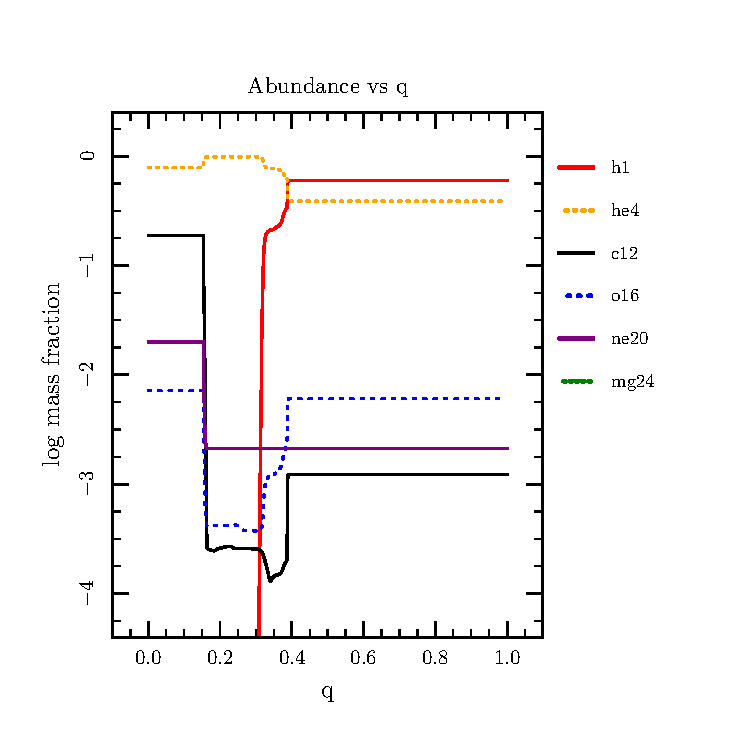
\includegraphics[width = 3.8in]{/Users/jaredbrooks/irradiated_planet/plots_out/Abundance_vs_q_5.pdf}
		       \caption{Abundance profile shows full convection}
		       \label{fig:1}
                \end{minipage}
                \hspace{0cm}
                \begin{minipage}[b]{0.5\linewidth}
                       \centering
                       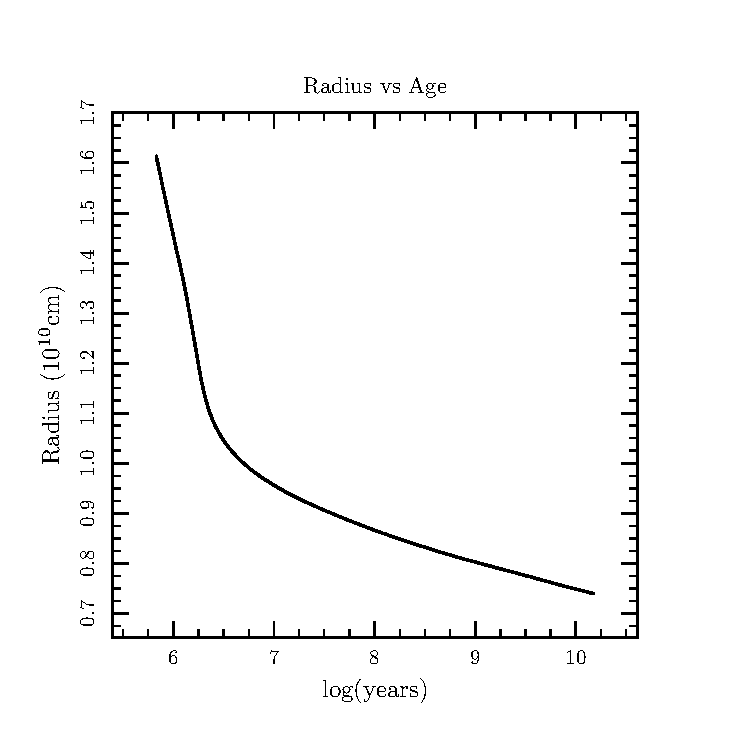
\includegraphics[width = 3.8in]{/Users/jaredbrooks/irradiated_planet/plots_out/logR_vs_log_Age.pdf}
                       \caption{Contraction of planet}
                       \label{fig:2}
                \end{minipage}
	\end{figure}

        \pagebreak

        To the left is log[g] vs effective temperature plot (figure \ref{fig:3}) to show the surface properties of the planet.  To the right is center temperature vs center density plot (figure \ref{fig:4}) showing the properties at the center of the planet.  Both show trends of general contraction and cooling.

        \begin{figure}[H]
                \begin{minipage}[b]{0.5\linewidth}
                       \centering
                       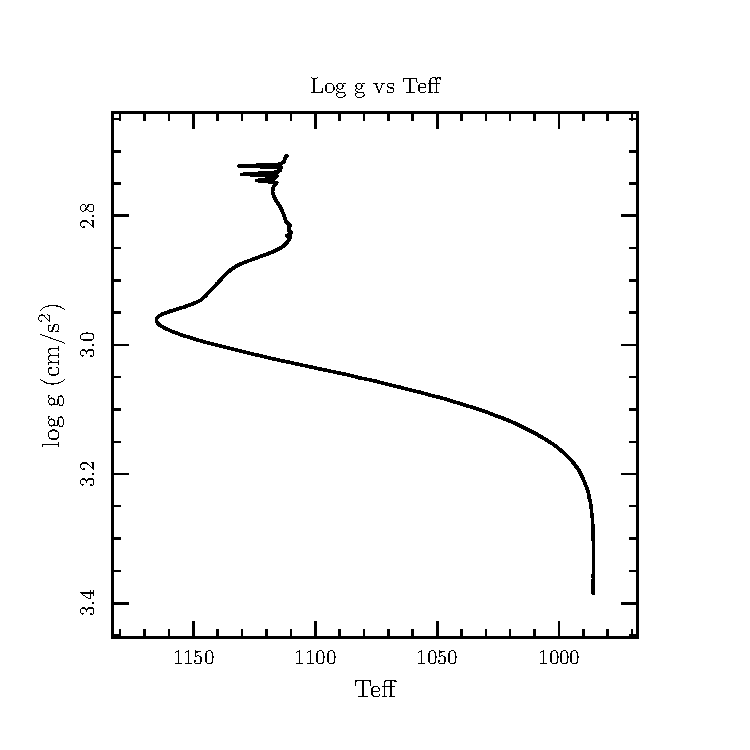
\includegraphics[width = 3.8in]{/Users/jaredbrooks/irradiated_planet/plots_out/log_g_vs_Teff.pdf}
                       \caption{log[g] vs effective temperature}
                       \label{fig:3}
                \end{minipage}
                \hspace{0cm}
                \begin{minipage}[b]{0.5\linewidth}
                       \centering
                       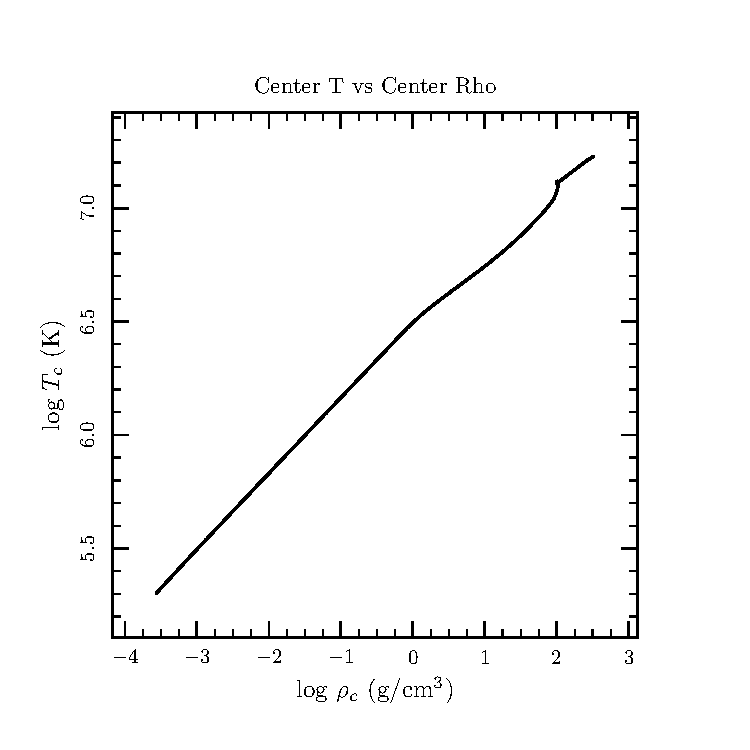
\includegraphics[width = 3.8in]{/Users/jaredbrooks/irradiated_planet/plots_out/Tc_vs_Rhoc.pdf}
                       \caption{Evolution of temperature and density at center of planet}
                       \label{fig:4}
                \end{minipage}
        \end{figure}

        \pagebreak

        Below is a temperature vs density profile taken at several different ages (figure \ref{fig:5}), with the red dots representing the top of the convection zones.  This shows that the planet is contracting and cooling until the surface temperature begins to approach the equilibrium temperature from irradiation and levels off.

        \begin{figure}[H]
                \centering
                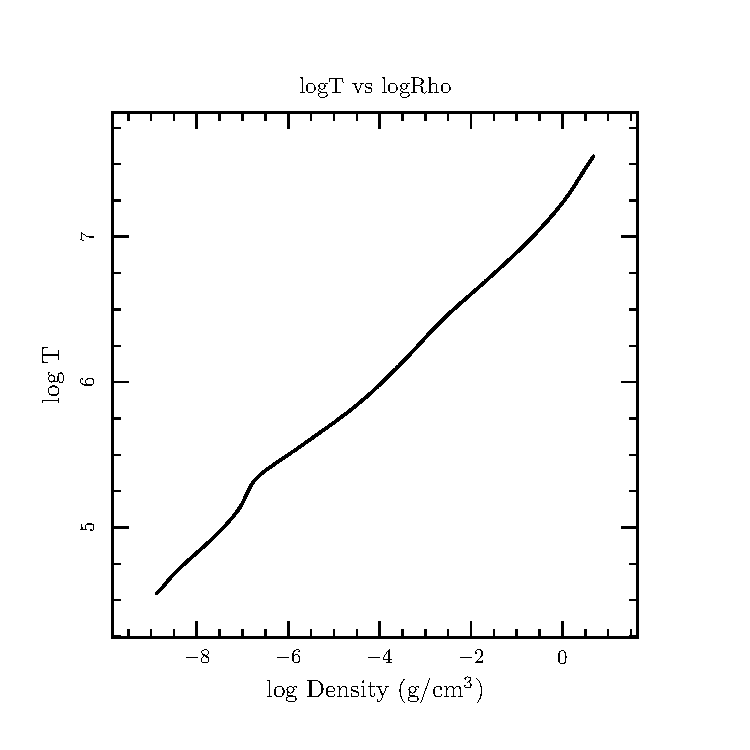
\includegraphics[width = 5in]{/Users/jaredbrooks/irradiated_planet/plots_out/Log_T_vs_logRho.pdf}
                \caption{Planet contracts and cools until surface nears equilibrium temperature, red dots are top of convection zone}
                \label{fig:5}
        \end{figure}

        \pagebreak

        This final plot (figure \ref{fig:7}) is meant to show a few internal \texttt{MESA} variables, such as the size of the time-step, the number of zones, and the number of retries against the model number in order to give some understanding of how hard \texttt{MESA} is working throughout the run and where some areas of problems/interest might be.

        \begin{figure}[H]
                \centering
                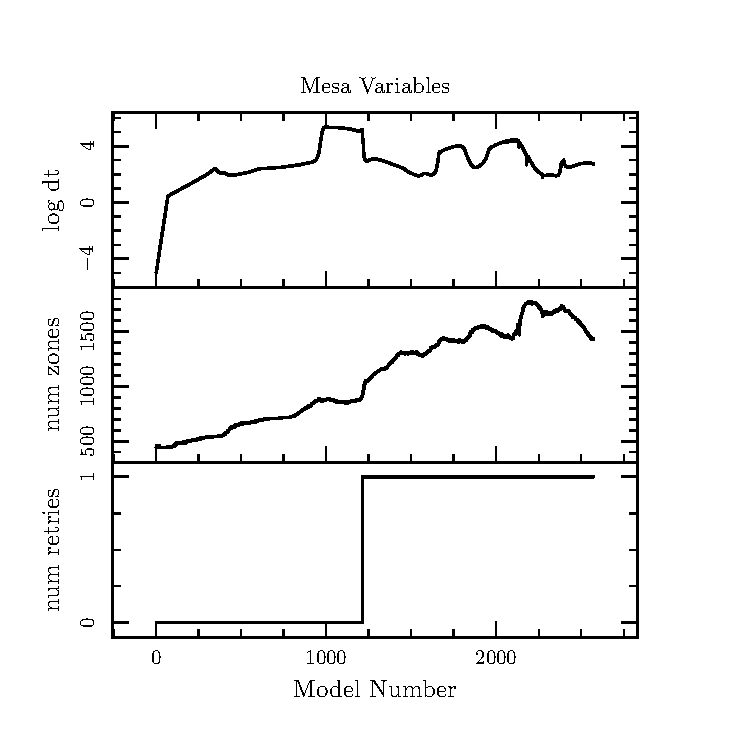
\includegraphics[width = 5in]{/Users/jaredbrooks/irradiated_planet/plots_out/Mesa_Variables.pdf}
                \caption{\texttt{MESA} variables plotted against model number show how hard \texttt{MESA} is working}
                \label{fig:7}
        \end{figure}

\end{document}


